% !TeX root = ../main.tex
% -*- coding: utf-8 -*-

\chapter{仿真实验与评估}

本文选择一种简单的民间纸牌游戏,来验证前面所提出的“自适应 Deep Q-Learning 算法”是否能够较为适应地处理现实中的实际问题。

\section{实验环境建立}

\subsection{纸牌游戏的背景与规则介绍}

在本游戏中共有三位玩家进行对战博弈,发牌前会从初始牌面中去掉 “红桃2”、“梅花2”、“方块2”、“黑桃A”这 4 张牌,共计 48 张牌,每人发牌 16 张。发牌后,第一回合由持手牌“黑桃3”的玩家出牌,随后依逆时针顺序跟牌,且要求在能出牌的情况下必须出牌,不可直接过牌。

作为第一位玩家出牌时,可任意选择牌型出牌,而跟牌阶段则只能按规则在指定牌型下出牌,最先将手牌出完的玩家为胜者。

该游戏规则简单,共有以下几种牌型:

\begin{center}
    \tablecaption{牌型介绍}
\begin{tabular}{c|c|c|c}
    \toprule[2pt]
    {\jiacu\heiti 牌型简称} & {\jiacu\heiti 牌型描述} & {\jiacu\heiti 牌型简称} & {\jiacu\heiti 牌型描述} \\
    % \midrule[2pt]
    \hline
    对子 & 两张相同的牌 & 三条 & 三张相同的牌 \\
    % \hline
    炸弹 & 四张相同牌 & 三带一 & 三条+单牌 \\
    % \hline
    三带二 & 三条+任意两张牌 & 单顺 & 至少5张的连续牌 \\
    % \hline
    双顺 & 至少2组连续对子 & 三顺 & 至少2组连续三条 \\
    % \hline
    飞机 & 至少2组连续三带二 & 四带二 & 炸弹+任意两张牌\\
    \bottomrule[2pt]
\end{tabular}
\end{center}

该纸牌游戏规则下,由于每轮出牌后具有动态不确定性,因此该游戏属于不完全信息博弈。

\subsection{模拟建立的纸牌游戏环境}

基于游戏的基本规则,使用 \texttt{Python} 编程语言构建了一个简单的游戏模拟环境。为了能够进行数值化的模型训练,需要将不同纸牌转化为对应的数值编号,具体地,将游戏规则下一副牌(该规则下共 48 张牌)从 “黑桃3” 到 “方块2” 由小到大对应为一个长度为 48 的一维向量,每张牌都有一个唯一的 ID ,例如 \texttt{['黑桃3', '黑桃5', '红桃5', '梅花5', '黑桃7']} 转化后应为 \texttt{[0, 8, 9, 10, 16]}。后面的实验介绍中,模型内部结构均基于此前提。

在 \texttt{utils.py} 文件中,定义了 \texttt{divide\_cards()} 函数来实现发牌功能,能够随机将 48 张牌分为三份,发放给三位玩家,每位玩家各自分配到长度为 16 的一维向量,代表自己的手牌。

同时还定义了 \texttt{calculate\_score()} 函数,它能够根据游戏规则来计分,起到向模型传递反馈奖励值的作用。

在 \texttt{RunFastGame.py} 中,定义了一个完整的 \texttt{RunFastGameEnv} 类,它能够完整地模拟卡牌游戏对局,其中 \texttt{RunFastGameEnv.get\_state()} 函数能够获得当前所处的状态 $s$,\texttt{RunFastGameEnv.play\_cards()} 能够接收策略传入的指令来采取相应的行动 $a$。

具体地,\texttt{RunFastGameEnv} 能够模拟卡牌游戏对局中的每位玩家,它能基于环境信息以及模型的策略决策情况来模拟完整的游戏对局,从而产生了真实的经验数据,提供给模型进行 Monte Carlo 模拟,从而得以实现之前提出的算法。

\section{算法仿真与评估}

\subsection{Deep Q-Network 算法实现细节}

在 \texttt{DQN.py} 中,定义一个 \texttt{QNet} 类,建立一个全连接神经网络,其深度为 4 层。输入层有 209 个神经元,对应输入特征向量的 209 个元素;隐藏层 1 有 512 个神经元;隐藏层 2 有 256 个神经元;隐藏层 3 有 128 个神经元;隐藏层 4 有 64 个神经元;输出层只有一个神经元,其输出值为 $Q$ 函数所对应的值。

在输入层和三个隐藏层之间都加入了 ReLU 线性整流单元\cite{li2017convergence}作为激励函数,其表达式为 $\mathrm{ReLU}(x) = \max(0,x)$。

同时也在这些连接层中加入了 DropOut 机制,它可以通过随机丢弃一些中间结果来有效防止过拟合\cite{srivastava2014dropout}。

完整的神经网络结构如下图所示:

\begin{figure}[H]
    \centering
    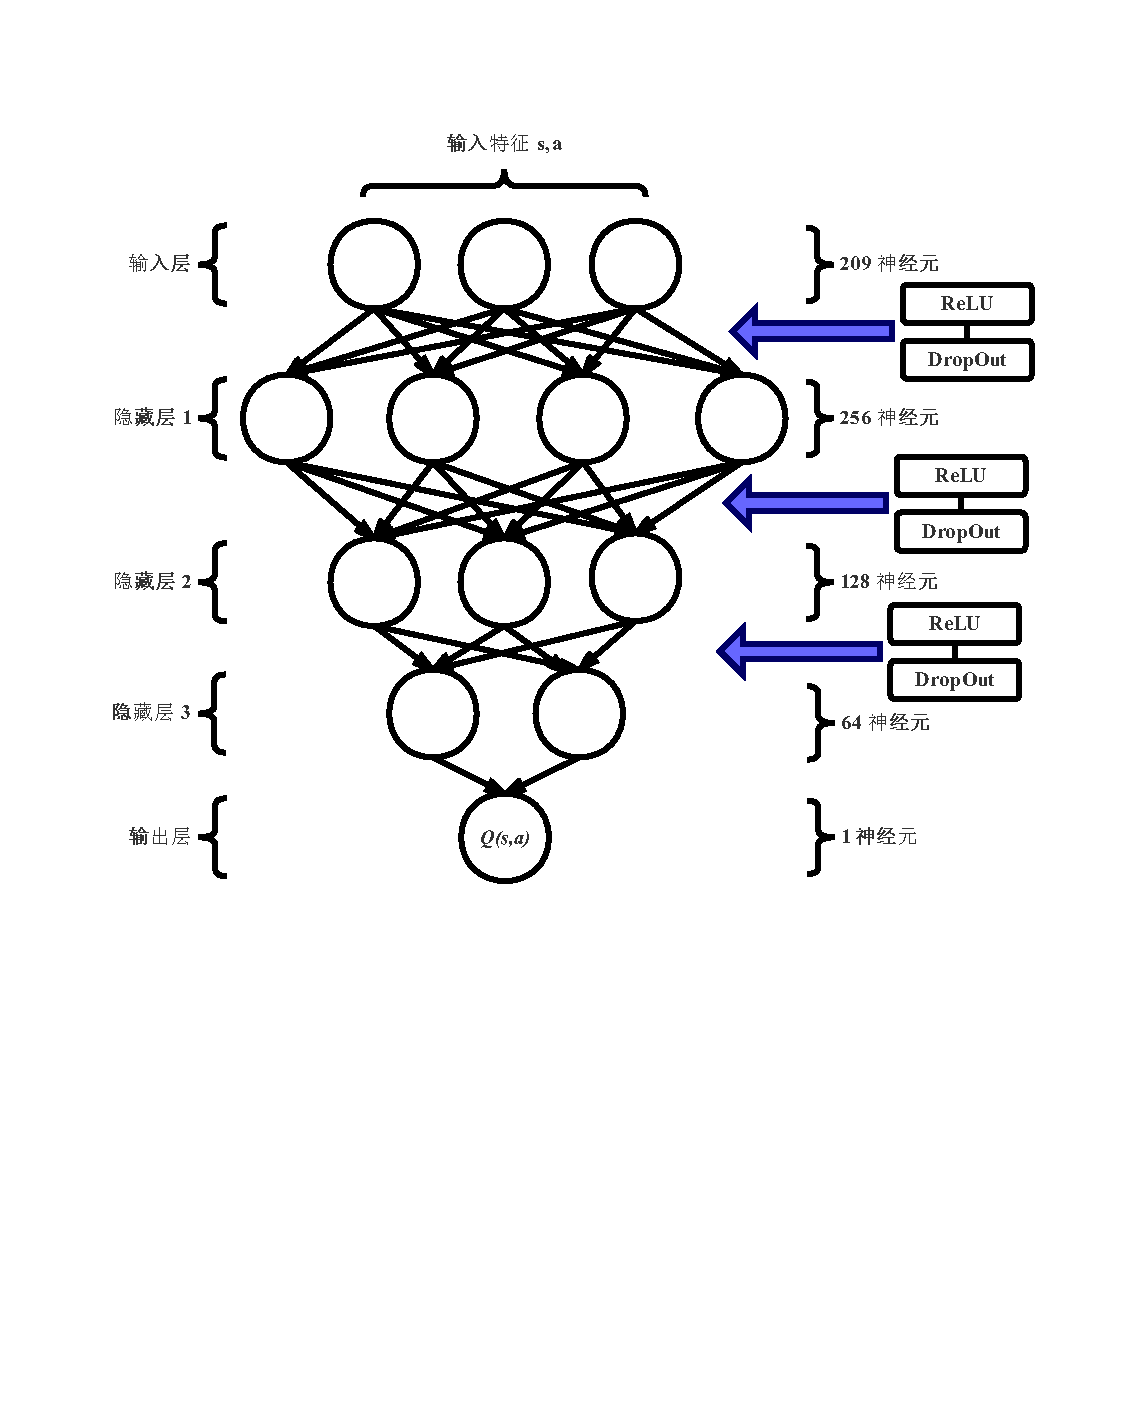
\includegraphics[width=0.9\textwidth]{DQN-Detail.pdf}
    \caption{Deep Q-Network 实现细节}
\end{figure}

在 \texttt{DQN.py} 中还定义了一个 \texttt{DQN} 类,用以实现 Deep Q-Learning 的细节。其中,\texttt{DQN.choose\_action()} 函数代表策略函数 $\pi$ ,输入的状态 $s$ 后,根据 $Q$ 函数大小决定的策略概率分布 $\pi(a|s)$ 来决定下一步应采取的行动 $a$ ,其中

\begin{equation}
    \pi(a|s)=
    \begin{cases}
        \frac{\varepsilon}{|\mathcal A(s)|}&, a\neq\arg\max_aQ(s,a)\\
        1-\varepsilon-\frac{\varepsilon}{|\mathcal A(s)|}&, a=\arg\max_aQ(s,a)
    \end{cases}
\end{equation}

\texttt{DQN.store\_transition()} 函数和 \texttt{DQN.add\_reward()} 函数用于将模拟过程中的一些关键信息存储于缓存中.

\texttt{DQN.learn()} 函数的作用是将缓存的信息提取出来,通过神经网络进行 Q-Learning 更新,更新公式为

\begin{equation}
    \widehat{Q}(S_t,A_t,\boldsymbol{w})\leftarrow \widehat{Q}(S_t,A_t,\boldsymbol{w})+\alpha\left[R_{t+1}+\gamma  \max\limits_a \widehat{Q}(S_{t+1},a,\boldsymbol{w})-\widehat{Q}(S_t,A_t,\boldsymbol{w})\right]
\end{equation}

最后,将 Deep Q-Network 模型接入进前面构建好的 \texttt{RunFastGameEnv} 环境下,即可开始模拟和训练的过程。

\subsection{仿真实验细节}

在前面所建立的仿真实验环境 \texttt{RunFastGameEnv} 中,由于是三人不完全信息博弈,即有 $N=3$,故总共需要建立六个 Deep Q-Network,每位玩家分配两个神经网络。

由于自适应 Deep Q-Learning 算法能够抵消估计偏差值,因此可以使用风格不同的三位玩家模型进行博弈训练,而风格差异化能够增加训练模型的鲁棒性,增强模型处理不确定性状态的能力。记三名玩家为分别为 $A,B,C$ ,其中 $A$ 玩家对应的模型为主训练模型,玩家 $B,C$ 为辅助学习模型,通过调整贪心率 $\varepsilon$ 使得辅助学习模型的决策水平与主训练模型形成差异化。其中 $\varepsilon_B = \varepsilon_A / 2$ ,$\varepsilon_C = \varepsilon_A / 3$。

此外,为了加速强化学习的学习效率,将算法中的贪心学习率 $\varepsilon$ 进行了动态调整,从初始值 $\varepsilon_0 = 0.4$ 随训练次数线性下降,每个 epoch 下降 0.01,达到预设的下限阈值 $\varepsilon_{stop} = 0.08$ 后停止动态调整。

基于前面所描述的细节,本实验的具体流程如下:

\begin{algorithm}[H]
    \caption{训练过程}
    \begin{algorithmic}[1] %每行不显示行号
        \State 初始化三名水平不同的玩家 $A, B, C$
        \Repeat
        \State 开始新一局游戏,并为三名玩家发牌
        \Repeat
        \State 根据游戏规则决定当前回合应当出牌的玩家
        \State 进入当前玩家的视角,根据场面信息获取当前所处状态 $S$
        \State 将状态 $S$ 传入 $Q$ 函数 和 $\pi$ 策略,决策下一步所要采取的行动 $a$
        \State 实际采取行动 $a$ ,接收环境传递的反馈值,并存入缓存
        \Until{执行行动 $a$ 后本局游戏分出胜负}
        \State 根据游戏规则,统计该局游戏各玩家得分,并追加存储至缓存
        \State 将缓存的信息,作为输入参数传入神经网络
        \State 经由神经网络完成一次训练学习,得到新的 $Q$ 函数和 $\pi$ 策略,用于下一次决策
        \Until{达到预设的训练次数}
        \State 结束训练,输出训练所得到的模型和参数
    \end{algorithmic}
\end{algorithm}

实验的完整流程图如下所示:

\begin{figure}[H]
    \centering
    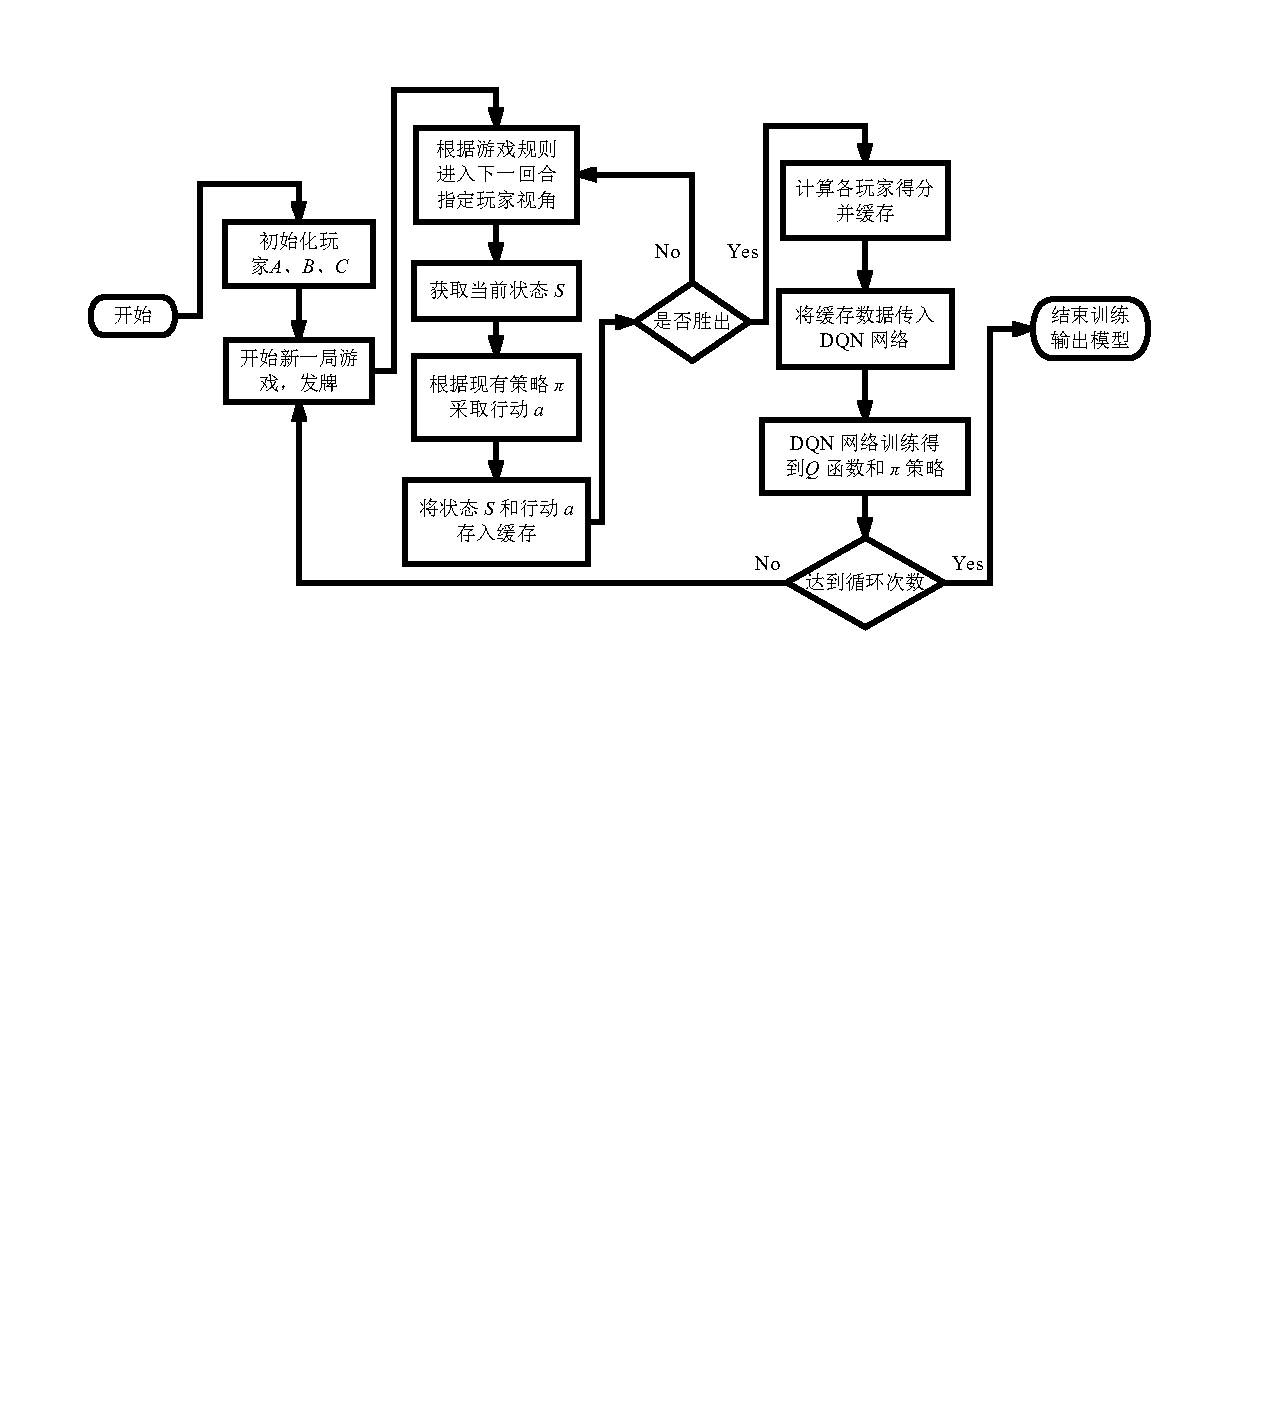
\includegraphics[width=\textwidth]{DQN-Process.pdf}
    \caption{实验流程图}
\end{figure}

\section{仿真实验结果与分析}

在 $\mathrm{NVIDIA}^\circledR$ GTX 1080 GPU 的硬件条件下,经过 100 万余局自我对战学习(其中每 2000 局作为一个 epoch 集中学习),最终决策函数 $Q$ 得到如下图所示的收敛情况。

\begin{figure}[H]
	\centering
	\begin{subfigure}{0.49\textwidth} % width of left subfigure
		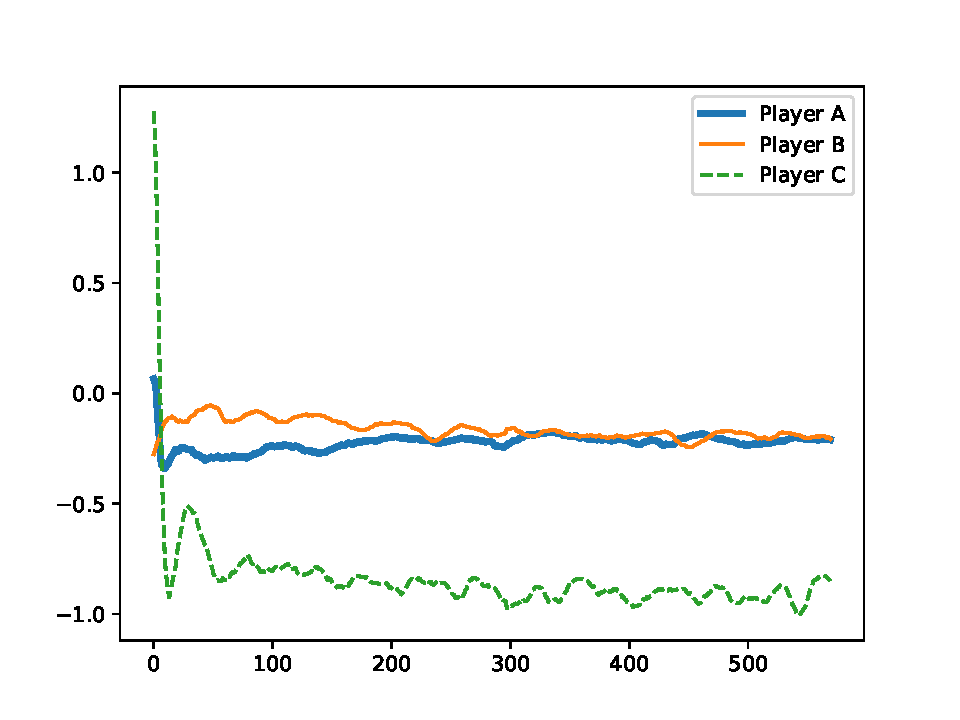
\includegraphics[width=\textwidth]{q-value.pdf}
		\caption{Q 函数训练均值}\label{img:q-value} % subcaption
	\end{subfigure}
	\vspace{1em} % here you can insert horizontal or vertical space
	\begin{subfigure}{0.49\textwidth} % width of right subfigure
		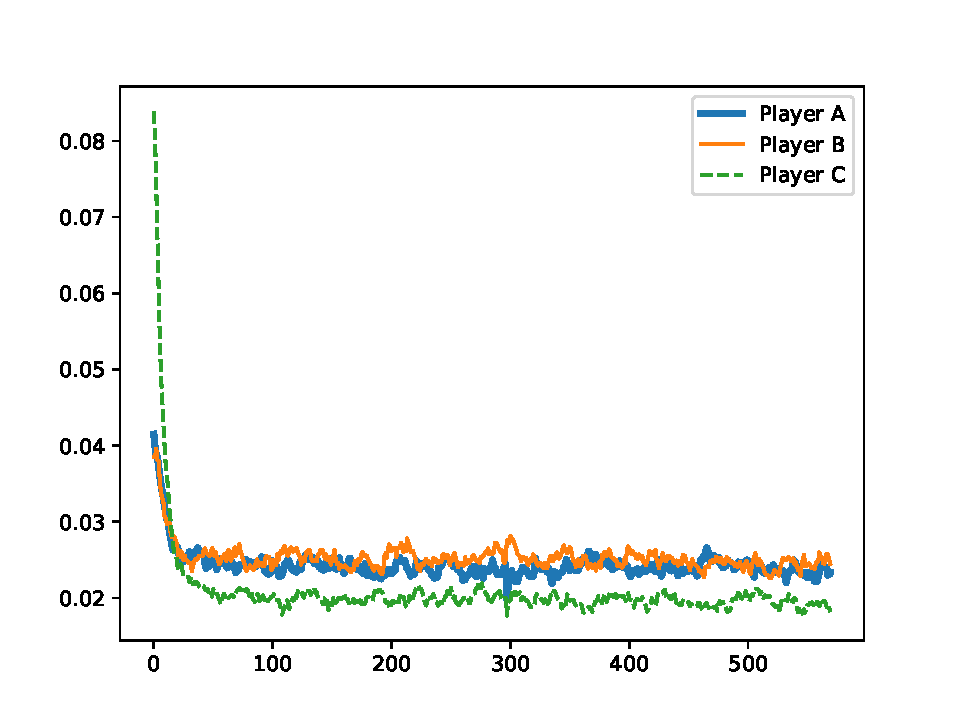
\includegraphics[width=\textwidth]{train-loss.pdf}
		\caption{Q-Learning 训练误差值}\label{img:train-loss} % subcaption
	\end{subfigure}
	\caption{仿真实验的训练结果} % caption for whole figure
\end{figure}

图\ref{img:q-value}刻画的是 Q 函数随训练次数的均值,观察可知经过该算法训练可使行动价值函数 $Q(s,a)$ 收敛,进而可以得到 $\varepsilon$-贪心策略:

\begin{equation}\label{eq:epspolicy}
    \pi(a|s)=
    \begin{cases}
        \frac{\varepsilon}{|\mathcal A(s)|}&, a\neq\arg\max_aQ(s,a)\\
        1-\varepsilon-\frac{\varepsilon}{|\mathcal A(s)|}&, a=\arg\max_aQ(s,a)
    \end{cases}
\end{equation}

其中策略 $\pi(a|s)$ 是一个条件概率分布,其含义是模型处于状态 $s$ 时,决定采取行动 $a$ 的概率。

另外,也可根据训练中的损失函数观察其收敛效果,图\ref{img:train-loss}所示的即为 自适应 Deep Q-Learning 算法的梯度损失项:

\begin{equation}
    \centering
    J(\boldsymbol{w}) = \frac{1}{2}\left[R_{t+1}+\gamma\max_a\widehat{Q}(S_{t+1},a,\boldsymbol{w})-\widehat{Q}(S_t,A_t,\boldsymbol{w})\right]^2
\end{equation}

从图中可观察知,损失项最后下降至一个较小值,Q 函数逐渐收敛。

\begin{figure}[H]
    \centering
    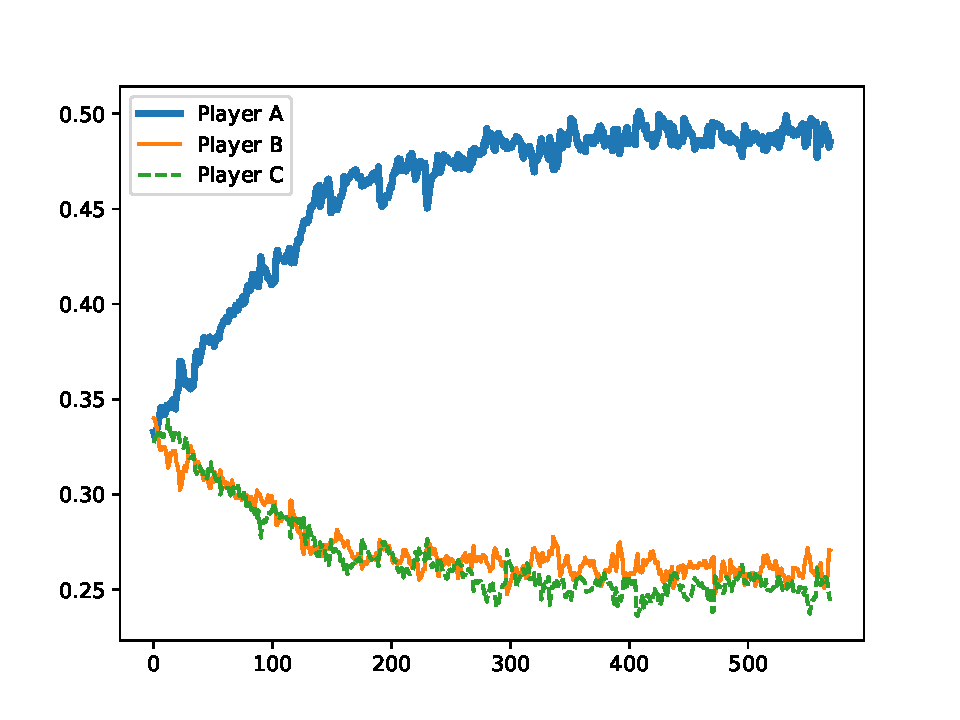
\includegraphics[width=0.57\textwidth]{win-rate.pdf}
    \caption{Q 函数与实时训练胜率}\label{img:win-rate}
\end{figure}

图\ref{img:win-rate}展现了三个玩家模型在训练中的实时胜率,观察发现其在训练过程中,自适应 Deep Q-Learning 算法的主训练模型胜率不断上升,远优于另外两个辅助学习模型,显然自适应 Deep Q-Learning 算法通过强化学习的思想学习和掌握了一定程度的游戏技巧。

为了验证自适应 Deep Q-Learning 的实际学习效果,使用训练出的策略模型进行了独立测试,通过调整算法中的贪心率 $\varepsilon$ ,从而影响到最终的实际决策策略 $\pi$ ,如\ref{eq:epspolicy}式所示。独立测试的结果如下:

\begin{table}[H]
\caption{独立测试结果}
\begin{center}
\scalebox{0.8}{
\begin{tabular}{cc|cc|cc}
    \toprule[2pt]
    \multicolumn{2}{c|}{主模型 A}&\multicolumn{2}{c|}{辅助模型 B}&\multicolumn{2}{c}{辅助模型 C}\\
    \hline
    \multicolumn{1}{c|}{$1-\varepsilon_A$}&\multicolumn{1}{c|}{胜率}&\multicolumn{1}{c|}{$1-\varepsilon_B$}&\multicolumn{1}{c|}{胜率}&\multicolumn{1}{c|}{$1-\varepsilon_C$}&\multicolumn{1}{c}{胜率}\\
    \hline
    0.99&0.662&0.99&0.165&0.99&0.173\\
    0.99&0.685&0.90&0.158&0.90&0.157\\
    0.95&0.621&0.80&0.191&0.80&0.188\\
    0.95&0.646&0.70&0.173&0.70&0.181\\
    0.90&0.558&0.60&0.221&0.60&0.221\\
    0.90&0.583&0.50&0.207&0.50&0.210\\
    \bottomrule[2pt]
\end{tabular}}
\end{center}
\label{tab:testresult}
\end{table}

基于独立测试结果,发现主训练模型在各种贪心率下相比于辅助训练模型均有着明显的策略优势,因此可以得出结论:自适应 Deep Q-Learning 算法能够有效处理不完全信息博弈问题。